\section{Validation}

We use a transition anchor position of
%$$t_-(n) =  t(n) \frac{ b^{-1}(n) - p(n) }{p(n+1) - p(n) }$$
%$$t_-(n) =  t(n) \frac{ b^{-1}(n) - 0.4n }{0.4(n+1) - 0.4n }$$
%$$t_-(n) =  t(n) \frac{ b^{-1}(n) - 0.4n }{0.4}$$
$$t_0(n) =  t(n) \left( b^{-1}(n) / 0.4  - n \right)$$
This should ensure that the transitions never overlap with the locations $v$ where $2 R(v) = 0.4n$ for $n \in \mathbb{N}$, since \SI{0.4}{\milli\meter} is the prefered bead width for a similar nozzle size.

$$d_\text{max}^\text{transition} = \SI{1}{\milli\meter}$$
$$d^\text{discretization} = \SI{0.2}{\milli\meter}$$
$$t_\text{beading} = \SI{0.4}{\milli\meter}$$
$$d_\text{max} = \SI{75}{\percent}$$


\subsection{Strategies}
We can emulate a variety of toolpath generation strategies by applying various beading strategies to our framework.

\paragraph{Naive Strategy}


\paragraph{Constant bead count}
Emulates \cite{Ding2016a}


\paragraph{Deviation at middle}
Emulates \cite{Jin2017}


\paragraph{Only outer bead}
Emulates \cite{Moesen2011}


\paragraph{Distributed strategy}
Distribute the overfill or underfill which would happen using a naive strategy over all beads.
This maximizes robustness and minimizes narrow beads qhich are difficult to print.


\paragraph{Combined strategy}
\Cref{wedge_and_infill} shows a combined toolpath strategy.

\begin{figure}
\centering
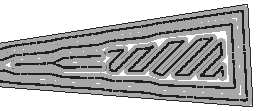
\includegraphics[width=.99\columnwidth]{sources/method/wedge_and_infill.pdf}
\caption{Use single and double wall lines in regions where the infill would be too thin.}
\label{wedge_and_infill}
\end{figure}





\subsubsection{Proposed optimal beading strategy}
@Readers: you can skip reading this section for now.
\todo{This section is about some optimal strategy which hasn't been fully developed (yet?).}
\todo{This section still formules the beading strategy in terms of radius instead of diameter, which halves the $n$ values.}

We need a function $W$ from a given radial distance $R(v)$ to a number of beads and their widths.
These widths depend on the following parameters:
\begin{description}
\item[$\wmin$] the minimum possible bead width
\item[$\wmax$] the maximum possible bead width
\item[$\wout$] the preferred bead width of the outer inset
\item[$\win$] the preferred bead width of the other insets
\end{description}

The function $W$ needs to be able to deal with a range which is considerably shorter than $[\wmin, 2\wmin]$, even so short as to accomodate just $[\win,\win]$ only.
The function needs to be such that we never overshoot the radial distance $R(v)$, because that would affect the dimensional accuracy.
Any distance left over which cannot be filled given the range $[\wmin, \wmax]$ should be placed on the inside near the MAT.

We define $W(d)$ as a sequence of bead widths.
The length of that sequence is $b(d)$.
For example: with $\win = \SI{0.4}{\milli\meter}$ we could have $b(1.05) = 2.5$ and $W(1.05) = (0.4, 0.4, 0.5)$.
The last number is the innermost bead width if there is a singleton bead along the medial axis; only half of that bead spans along a radial distance.

The function $b$ should adhere to several criteria:
\begin{itemize}
\item $b \left( \frac12 n\win \right) = \frac12 n$ for integer $n$
%\item $b$ is monotonic
%the item below follows from the two above
% \item between a location with radial distance $R(v) \in [\frac12 n\win, \frac12 (n+1)\win]$ (for integer $n$) there is only one transition to a different number of beads
\item $ 0 \leq b(d) \leq d / w_\text{min} $
%\item the width $W(c, d)_n$ of each bead $n$ increases monotonically and gradually in regions with constant bead count $c$: $0 \leq \frac{\partial W(c, d)_n}{\partial d} < \infty$.
\end{itemize}


For our application we define a $W$ adhereing to the following aditional constraints in order of priority:
\begin{itemize}
\item Minimize unfilled area
\item Try to get the outer bead width $W_1$ as close as possible to $\wout$
\item Have the rest of the $W_n$ the same width
\item at transition regions decide between $n$ and $n+1$ beads using the Loss fuction scheme below
\item From a $d$ for which $b(d) = 3$ we don't consider fractional $b(d)$ anymore; we don't allow singleton beads along the medial axis.
\hl{Perhaps we should disallow this because that would require a different transition length}
\end{itemize}

\iffalse
\begin{align}
W(d)_1 = 
  \begin{cases} 
%  \infty & \text{if } w < w_\text{min} \\
   \wout & \text{if } d \geq \wout + \wmin \\
   w - \wmin  & \text{if } 2\wmin  \leq d < \wout + \wmin
  \end{cases}
\end{align}
\fi

%\subsubsection{Optimal beading strategy}
%We could decide on a beading strategy based on some loss function $L$ defined on each line width.

\begin{align}
L(w_1) &= 
  \begin{cases} 
%  \infty & \text{if } w < w_\text{min} \\
   (w - \wout) / (\wmax - \wout) & \text{if } w > \wout\\
   (\wout - w) / (\wout - \wmin)       & \text{otherwise}
  \end{cases}
  \\
L(w_n) &= 
  \begin{cases} 
%  \infty & \text{if } w < w_\text{min} \\
   (w - \win) / (\wmax - \win) & \text{if } w > \win\\
   (\win - w) / (\win - \wmin)       & \text{otherwise}
  \end{cases}
\\
L(W(d)) &= \left(b(d) - \lfloor b(d) \rfloor \right) L \left( W(d)_{\lceil b(d) \rceil} \right)  +  \sum_{n=1}^{n=\lfloor b(d) \rfloor} L( W(d)_n )
\end{align}

(Singular beads are counted only half.)
Together these prioritized constraints uniquely define a single $W$, depending on $\wmin, \wmax, \wout,\win$.
An example is given in \cref{transition_location}.

\begin{figure*}
\centering
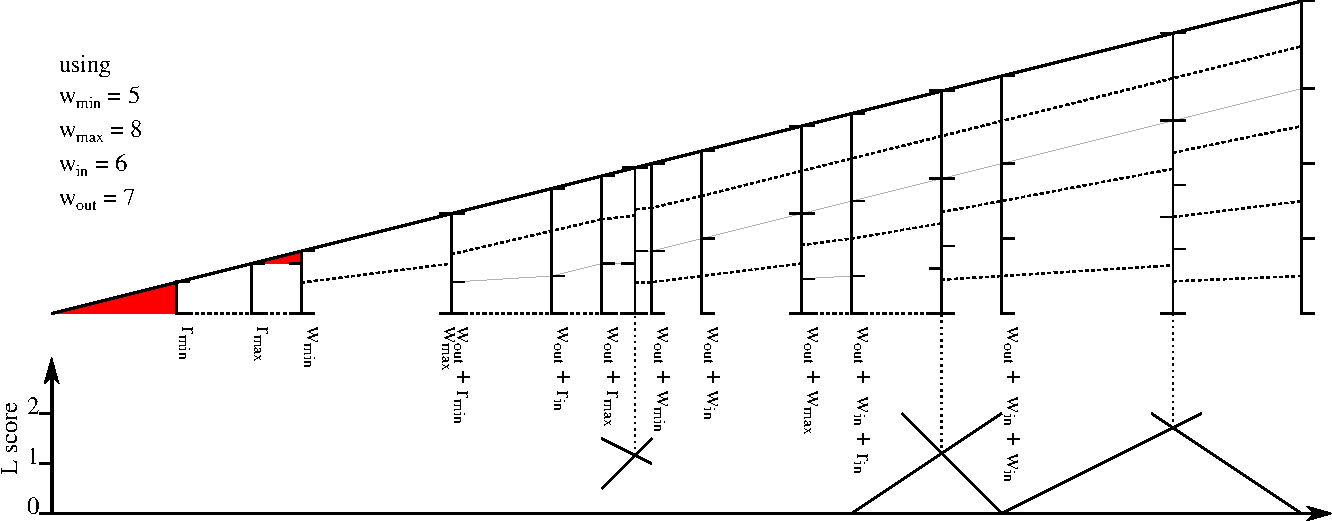
\includegraphics[width=.9\textwidth]{sources/method/ticking_v2.pdf}
\caption{Mapping of different lengths to a ticking. Transition location on a line-line segment is to the right of the middle because the preferred line width is to the left of the middle in the range.}
\label{transition_location}
\end{figure*}

The prefered width $p$ is given as follows:
\begin{align}
p(n) =
  \begin{cases} 
   \frac12 \wout & \text{if } n = \frac12 \\
    \wout + (n - 1) \win       & \text{otherwise}
  \end{cases}
\end{align}







\subsection{Computational analysis}
\paragraph{Accuracy}
Render toolpaths and calculate amount of overfilling and amount of underfilling.

\paragraph{Printability}
Define some function to determine printability $0<P<1$, 
then define a loss function $L = 1/P$.
Evaluate average loss divided by total toolpath length.

\old{Visualize thickness of beads as color.}

Show results for different settings.

\old{Also render with nozzle size as minimal width and use middle of toolpaths instead of middle of beads.}

Example shapes:
\begin{itemize}
\item same as Moessen: grids of triangular holes
\item same as Moessen: circular holes.
\item same as Jin 
\item same as Kao
\item wedge
\item layer of a typical model: phone case
\item some of the above shapes, but with some fuzzy randomized outline
\end{itemize}





\subsection{Experimentation}
Print objects and show qualities:
\begin{itemize}
\item visual consistency of flat top skin surface
\item visual gradual transparency changes
\item graphs of tensile tests on thin walled object
\end{itemize}

Print on mississipi?

What material should I print with for the tensile tests?









